\documentclass[a4paper,12pt]{article}

% ---------------------------------------------------------------------------
% ─── PAQUETES BÁSICOS ───────────────────────────────────────────────────────
% ---------------------------------------------------------------------------
\usepackage[utf8]{inputenc}
\usepackage[T1]{fontenc}
\usepackage[spanish]{babel}
\usepackage{graphicx}
\usepackage{subcaption}
\usepackage{caption}
\usepackage{listings}
\usepackage{amsmath}
\usepackage{float}
\usepackage{geometry}
\usepackage{fancyhdr}
\usepackage[hidelinks]{hyperref}
\usepackage{cleveref}

% ---------------------------------------------------------------------------
% ─── CONFIGURACIÓN GLOBAL ───────────────────────────────────────────────────
% ---------------------------------------------------------------------------
\geometry{margin=2.5cm}
\graphicspath{{images/}}          % <-- todas las figuras están en images/
\pagestyle{fancy}
\fancyhf{}
\lhead{GINI + Ensamblador + GDB}
\rhead{TP Sistemas de Computación}
\cfoot{\thepage}

% ---------------------------------------------------------------------------
% ─── LISTINGS (OPCIONAL) ────────────────────────────────────────────────────
% ---------------------------------------------------------------------------
\lstset{
  basicstyle=\ttfamily\small,
  numberstyle=\tiny,
  numbers=left,
  stepnumber=1,
  frame=single,
  captionpos=b,
  language=[x86masm]Assembler,  % cambiar a 'C' cuando sea necesario
  keywordstyle=\color{blue},
  commentstyle=\itshape\color{gray!70},
  morekeywords={fld,fistp,add,leave,ret}
}

% ---------------------------------------------------------------------------
% ─── METADATOS ──────────────────────────────────────────────────────────────
% ---------------------------------------------------------------------------
\title{\textbf{Inspección del stack en llamadas a ensamblador\\(TP GINI)}}
\author{Agustín \and Grupo SdeC 2025}
\date{\today}

% ===========================================================================

\begin{document}

\maketitle

\section{Introducción}
Este informe demuestra, mediante \textbf{GDB}, cómo inspeccionar el
\textbf{stack} durante la llamada desde un programa \emph{C} de 32 bits a
una rutina en ensamblador (\emph{cdecl}).  
El caso de prueba convierte un valor flotante (índice GINI) a entero
(\texttt{floor}) y le suma~1.

\section{Entorno de trabajo}
\begin{itemize}
  \item \textbf{Arquitectura:} x86 (32 bits).
  \item \textbf{Compiladores:} GCC (\texttt{-m32}), NASM (\texttt{-f elf32}).
  \item \textbf{Depurador:} GDB.
  \item \textbf{Entrada:} un \texttt{float} leído desde \texttt{stdin}.
  \item \textbf{Función ASM:} \texttt{calculate\_gini\_int}.
\end{itemize}

\section{Inspección del stack}
\subsection{Estado previo a la llamada}
La \cref{fig:before} muestra el estado del stack y del registro \texttt{esp}
antes de ejecutar la llamada a ensamblador.

\begin{figure}[H]
  \centering
  \begin{subfigure}{0.48\textwidth}
    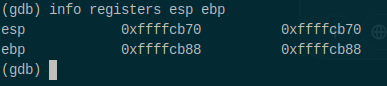
\includegraphics[width=\linewidth]{beforeasm.png}
    \caption{Registros \texttt{esp} y \texttt{ebp}.}
  \end{subfigure}
  \hfill
  \begin{subfigure}{0.48\textwidth}
    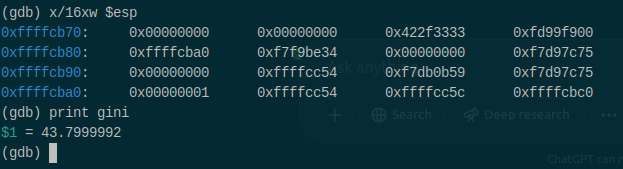
\includegraphics[width=\linewidth]{beforeasm2.png}
    \caption{Valor flotante en memoria (\texttt{0x422f3333} $\approx$ 43.8).}
  \end{subfigure}
  \caption{Estado del programa antes de la llamada a ASM.}
  \label{fig:before}
\end{figure}

\subsection{Ejecución en la rutina ASM}
La \cref{fig:asm} resalta las instrucciones críticas \texttt{fld},
\texttt{fistp}, y \texttt{add eax,\,1} dentro de la función.

\begin{figure}[H]
  \centering
  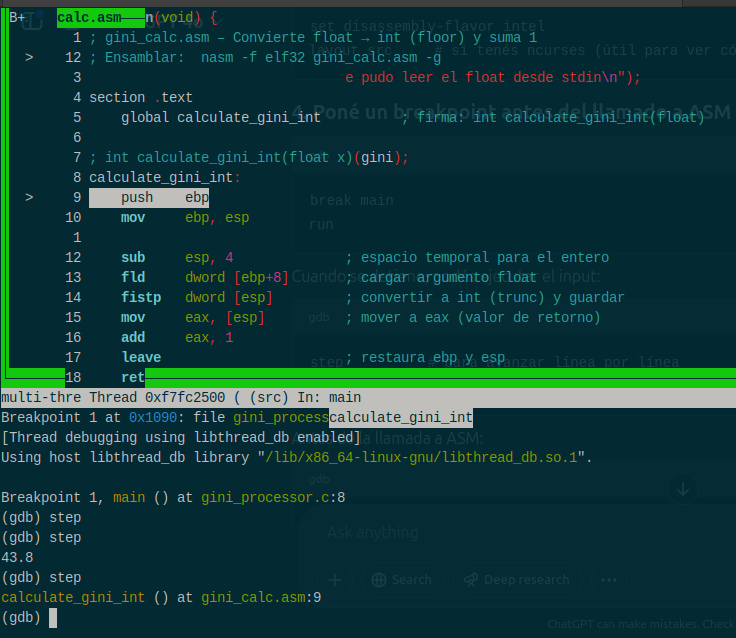
\includegraphics[width=0.75\textwidth]{calculategini.png}
  \caption{Vista paso a paso dentro de \texttt{calculate\_gini\_int}.}
  \label{fig:asm}
\end{figure}

\subsection{Retorno a \texttt{C}}
Tras el \texttt{ret}, el resultado entero reside en \texttt{EAX} y se copia a
\texttt{result} (\cref{fig:after}).  

\begin{figure}[H]
  \centering
  \begin{subfigure}{0.48\textwidth}
    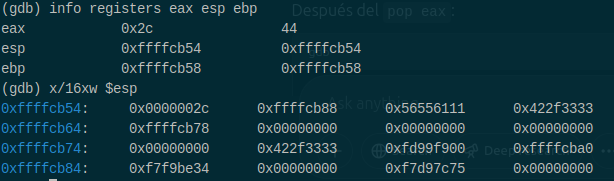
\includegraphics[width=\linewidth]{afterasm.png}
    \caption{\texttt{EAX} = 0x2D (45).}
  \end{subfigure}
  \hfill
  \begin{subfigure}{0.48\textwidth}
    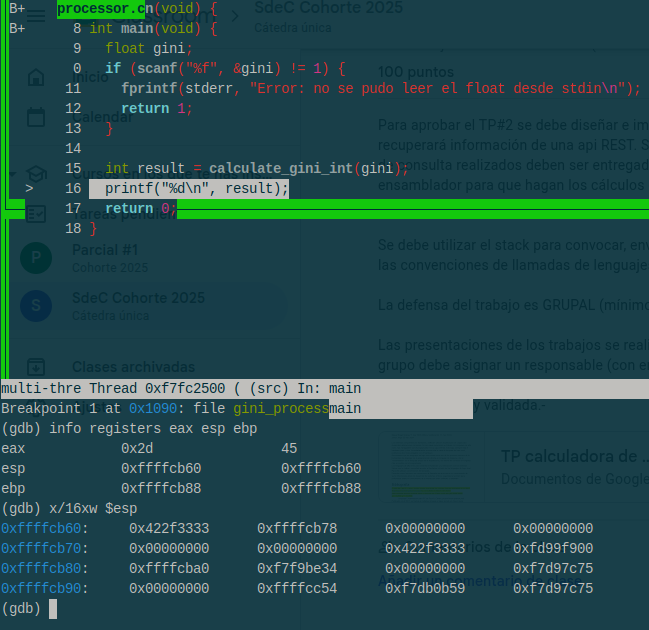
\includegraphics[width=\linewidth]{afterasm2.png}
    \caption{Variable \texttt{result} con el mismo valor.}
  \end{subfigure}
  \caption{Estado del programa después de la llamada.}
  \label{fig:after}
\end{figure}

Para mayor detalle, \cref{fig:eaxstack} muestra la dirección del
\texttt{float} en el stack y corrobora el valor devuelto.

\begin{figure}[H]
  \centering
  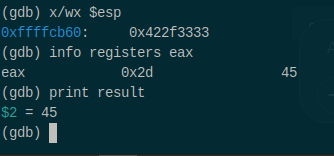
\includegraphics[width=0.55\textwidth]{ubicacionyvaloreax.png}
  \caption{Dirección del argumento y verificación de \texttt{EAX}.}
  \label{fig:eaxstack}
\end{figure}

\section{Diagrama de secuencia completo}
\begin{figure}[H]
  \centering
  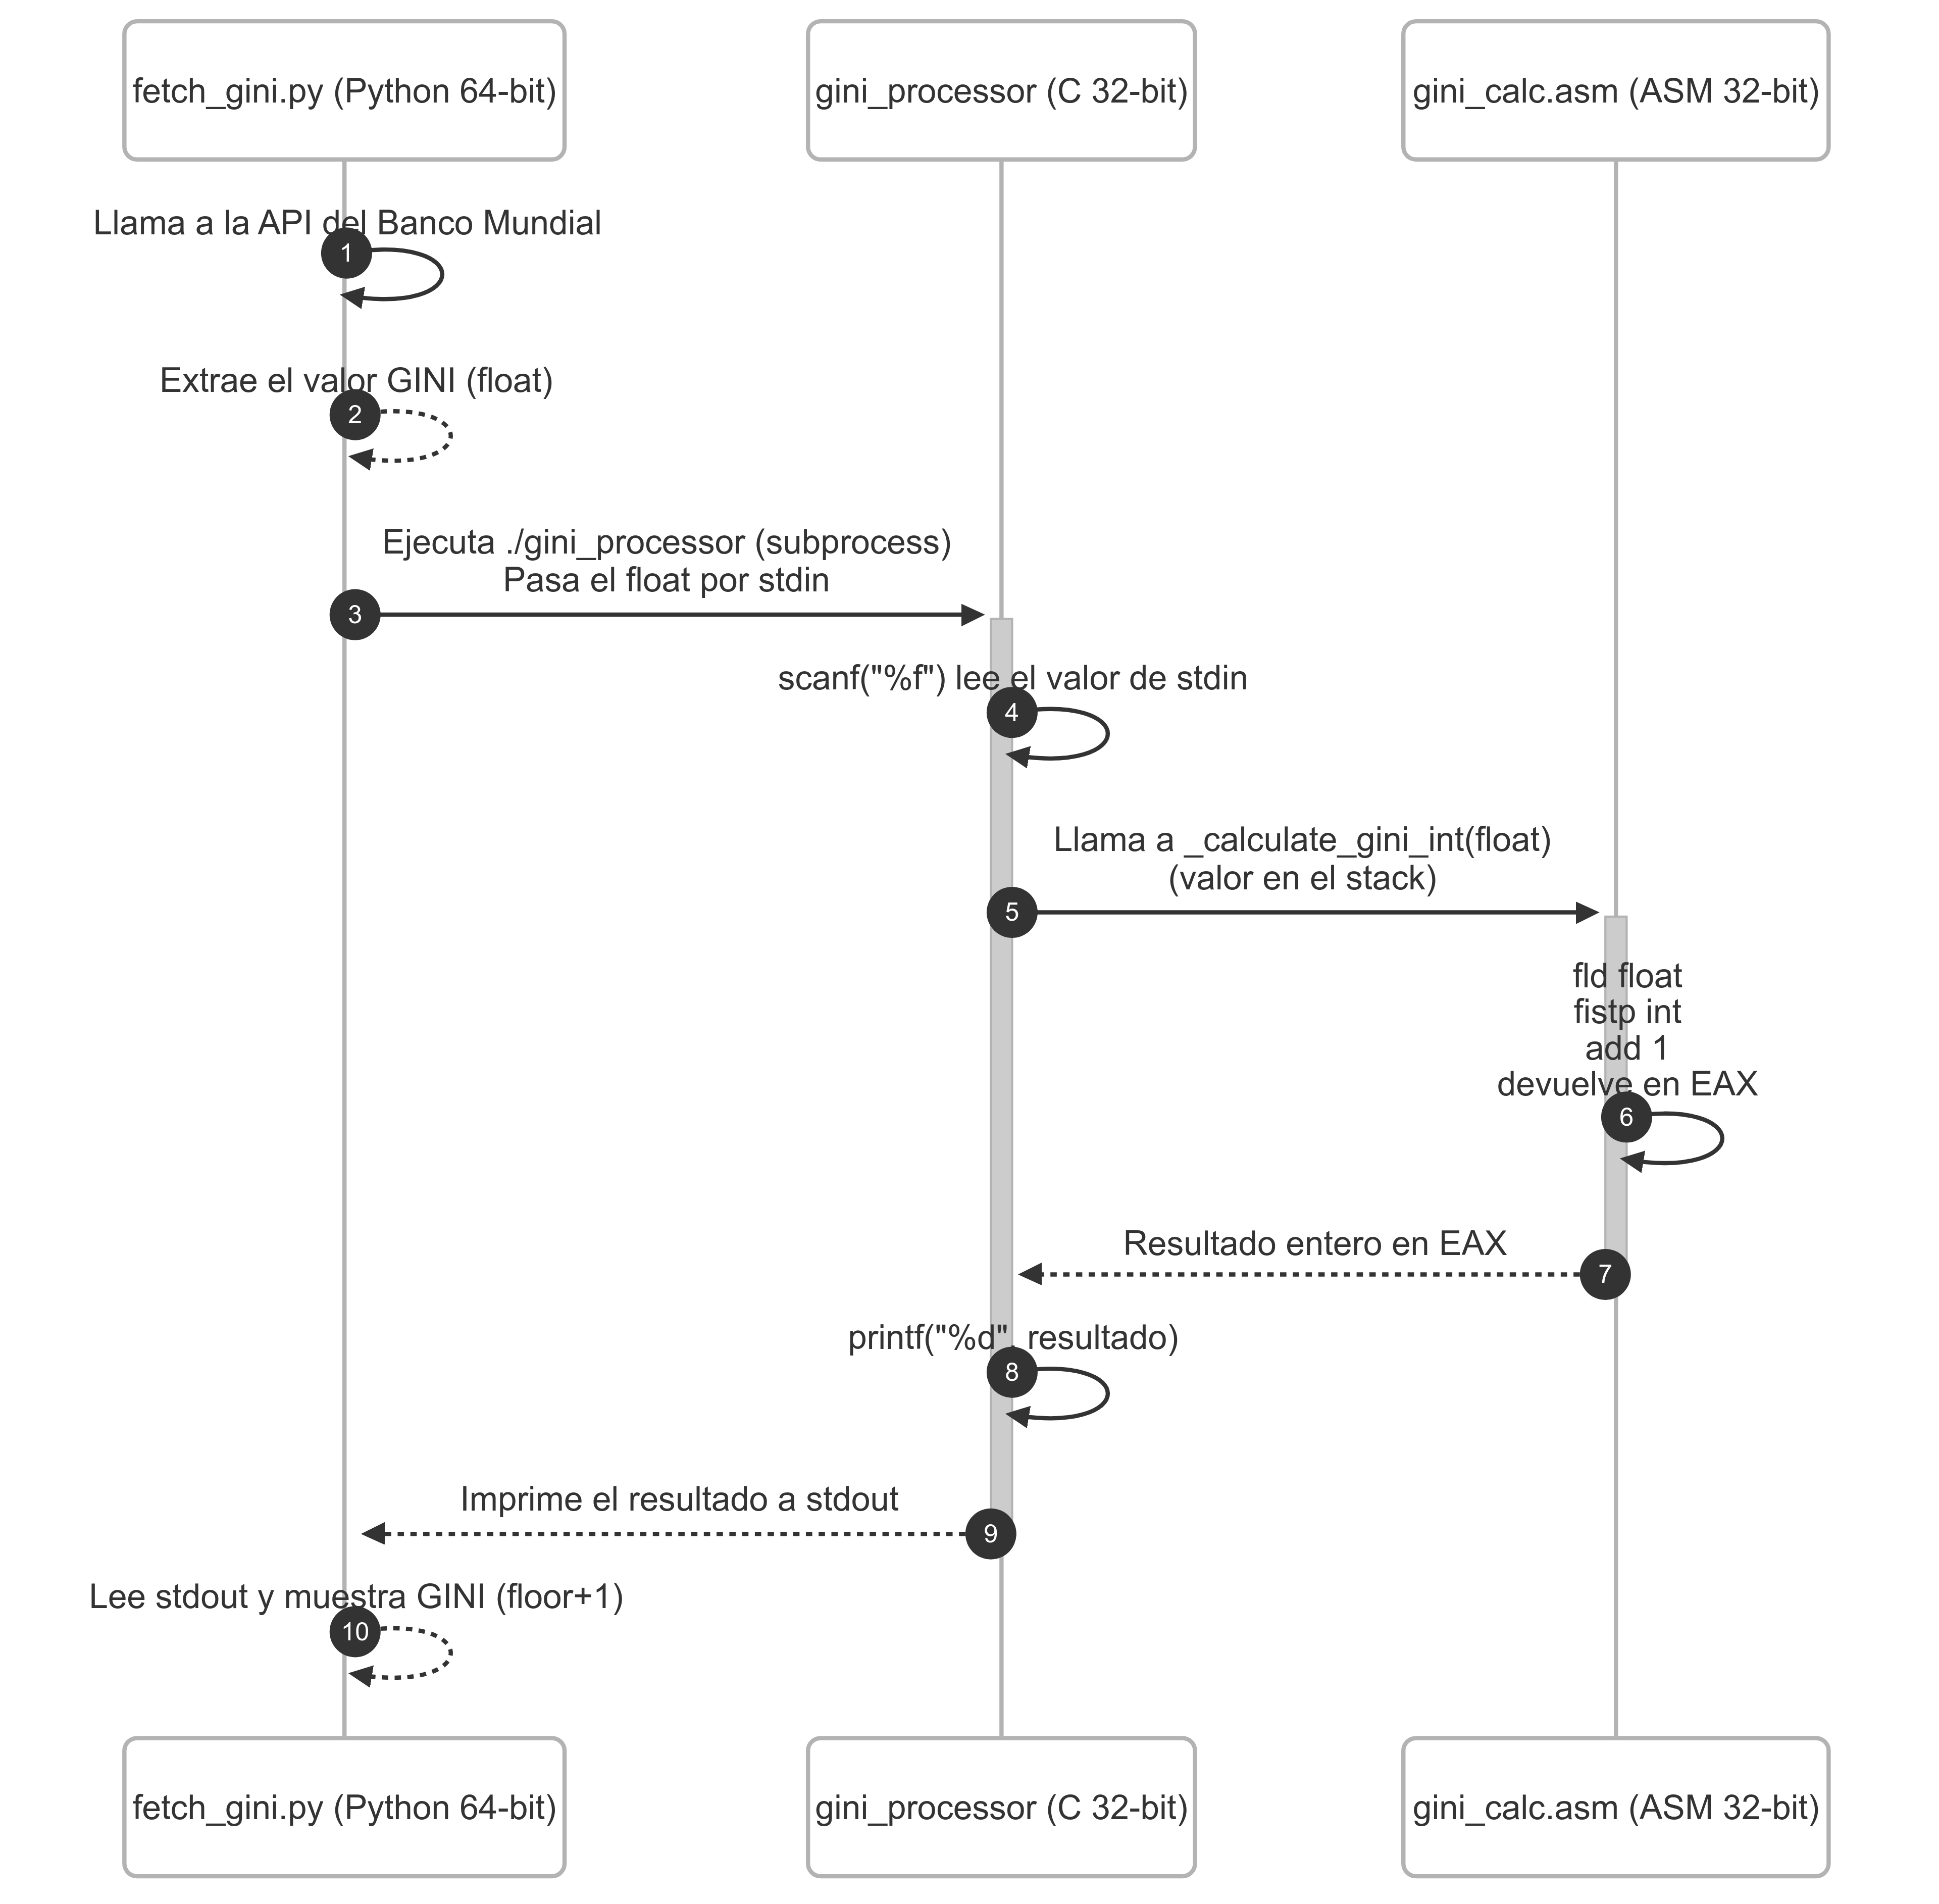
\includegraphics[width=0.9\textwidth]{diagram.png}
  \caption{Flujo end‑to‑end desde Python hasta la rutina ASM.}
  \label{fig:sequence}
\end{figure}

\section{Conclusiones}
GDB permitió rastrear el flujo de datos entre C y ensamblador:  
\textit{argumento en el stack $\rightarrow$ FPU $\rightarrow$ retorno en
\texttt{EAX}}.  La rutina en ASM cumple con la convención \emph{cdecl} y la
variable \texttt{result} refleja el valor correcto (GINI truncado + 1).

\end{document}
